%% Basierend auf einer TeXnicCenter-Vorlage von Mark Müller
%%%%%%%%%%%%%%%%%%%%%%%%%%%%%%%%%%%%%%%%%%%%%%%%%%%%%%%%%%%%%%%%%%%%%%%

% Wählen Sie die Optionen aus, indem Sie % vor der Option entfernen  
% Dokumentation des KOMA-Script-Packets: scrguide

%%%%%%%%%%%%%%%%%%%%%%%%%%%%%%%%%%%%%%%%%%%%%%%%%%%%%%%%%%%%%%%%%%%%%%%
%% Optionen zum Layout des Artikels                                  %%
%%%%%%%%%%%%%%%%%%%%%%%%%%%%%%%%%%%%%%%%%%%%%%%%%%%%%%%%%%%%%%%%%%%%%%%
\documentclass[%
%a5paper,							% alle weiteren Papierformat einstellbar
%landscape,						% Querformat
%10pt,								% Schriftgröße (12pt, 11pt (Standard))
%BCOR1cm,							% Bindekorrektur, bspw. 1 cm
%DIVcalc,							% führt die Satzspiegelberechnung neu aus
%											  s. scrguide 2.4
%twoside,							% Doppelseiten
%twocolumn,						% zweispaltiger Satz
%halfparskip*,				% Absatzformatierung s. scrguide 3.1
%headsepline,					% Trennline zum Seitenkopf	
%footsepline,					% Trennline zum Seitenfuß
%titlepage,						% Titelei auf eigener Seite
%normalheadings,			% Überschriften etwas kleiner (smallheadings)
%idxtotoc,						% Index im Inhaltsverzeichnis
%liststotoc,					% Abb.- und Tab.verzeichnis im Inhalt
%bibtotoc,						% Literaturverzeichnis im Inhalt
%abstracton,					% Überschrift über der Zusammenfassung an	
%leqno,   						% Nummerierung von Gleichungen links
%fleqn,								% Ausgabe von Gleichungen linksbündig
%draft								% überlangen Zeilen in Ausgabe gekennzeichnet
]
{scrartcl}

%\pagestyle{empty}		% keine Kopf und Fußzeile (k. Seitenzahl)
%\pagestyle{headings}	% lebender Kolumnentitel

%% Deutsche Anpassungen %%%%%%%%%%%%%%%%%%%%%%%%%%%%%%%%%%%%%
\usepackage[english]{babel}
\usepackage[T1]{fontenc}
\usepackage[utf8]{inputenc}

\usepackage{amsthm} % Theorem-Packet
\usepackage{amsmath}
\usepackage{amssymb}

\usepackage{stmaryrd} % Blitzsymbol
\usepackage{fancyhdr} % Für Kopfzeile
\usepackage{graphicx} % Einbinden von Grafiken
\usepackage{bbding} % Für das Häckchen
\usepackage{amscd} % Kommutative Diagramme
\usepackage{mathtools} % Für das Definitionssymbol

\usepackage{listings}
\usepackage{courier}

\pagestyle{fancy}
\lhead{Computational Science I}\chead{Exercise notes: Matrices}\rhead{HS 2013} % Kopfzeile

\newtheoremstyle{plain}%  name
  {.5\baselineskip}% Space above
  {.5\baselineskip}% Space below
  {}% Body font
  {}% Indent amount (empty = no indent, \parindent = para indent)
  {\bfseries}% Thm head font
  {:}% Punctuation after thm head
  { }% Space after thm head: " " = normal interword space; \newline = linebreak
  {}% Thm head spec (can be left empty, meaning `normal')
  
\makeatletter % Matrizen mit opitonalen Linien
\renewcommand*\env@matrix[1][*\c@MaxMatrixCols c]{%
  \hskip -\arraycolsep
  \let\@ifnextchar\new@ifnextchar
  \array{#1}}
\makeatother

\theoremstyle{plain}
\newtheorem*{bsp}{Beispiel} % Beispiele ohne Nummerierung
\newtheorem*{bws}{Beweis} % Beweise ohne Nummerierung 
\newenvironment{beweis}{\begin{bws}~\vspace{0.5\baselineskip}}{\hfill $\qedsymbol$\end{bws}}
\newenvironment{beispiel}{\begin{bsp}~\vspace{0.5\baselineskip}}{\end{bsp}}

\usepackage{lmodern} % Type1-Schriftart für nicht-englische Texte

\usepackage{enumerate}

\renewcommand\theenumi{\roman{enumi}}
\renewcommand\labelenumi{\theenumi)}

%% Packages für Grafiken & Abbildungen %%%%%%%%%%%%%%%%%%%%%%
%\usepackage{graphicx} %%Zum Laden von Grafiken
%\usepackage{subfig} %%Teilabbildungen in einer Abbildung
%\usepackage{tikz} %%Vektorgrafiken aus LaTeX heraus erstellen

%\setlength{\parindent}{0pt} % kein Einzug


%% Beachten Sie:
%% Die Einbindung einer Grafik erfolgt mit \includegraphics{Dateiname}
%% bzw. über den Dialog im Einfügen-Menü.
%% 
%% Im Modus "LaTeX => PDF" können Sie u.a. folgende Grafikformate verwenden:
%%   .jpg  .png  .pdf  .mps
%% 
%% In den Modi "LaTeX => DVI", "LaTeX => PS" und "LaTeX => PS => PDF"
%% können Sie u.a. folgende Grafikformate verwenden:
%%   .eps  .ps  .bmp  .pict  .pntg


%% Bibliographiestil %%%%%%%%%%%%%%%%%%%%%%%%%%%%%%%%%%%%%%%%%%%%%%%%%%
%\usepackage{natbib}

\begin{document}

\lstset{basicstyle=\ttfamily, breakatwhitespace=false, breaklines=true, frame=single, xleftmargin=\parindent, aboveskip=\baselineskip, belowskip=\baselineskip}

%\pagestyle{empty} %%Keine Kopf-/Fusszeilen auf den ersten Seiten.


%%%%%%%%%%%%%%%%%%%%%%%%%%%%%%%%%%%%%%%%%%%%%%%%%%%%%%%%%%%%%%%%%%%%%%%
%% Ihr Artikel                                                       %%
%%%%%%%%%%%%%%%%%%%%%%%%%%%%%%%%%%%%%%%%%%%%%%%%%%%%%%%%%%%%%%%%%%%%%%%

%% eigene Titelseitengestaltung %%%%%%%%%%%%%%%%%%%%%%%%%%%%%%%%%%%%%%%    
%\begin{titlepage}
%Einsetzen der TXC Vorlage "Deckblatt" möglich
%\end{titlepage}

%% Angaben zur Standardformatierung des Titels %%%%%%%%%%%%%%%%%%%%%%%%
\titlehead{\center{University of Zurich - HS 2013}}
%\subject{Typisierung}
\title{Computational Science I\\Exercise notes: Matrices\\\rule{1.0\textwidth}{1.0pt}}
\author{Tobias Grubenmann}
%\and{Der Name des Co-Autoren}
%\thanks{Fußnote}			% entspr. \footnote im Fließtext
%\date{}							% falls anderes, als das aktuelle gewünscht
%\publishers{Herausgeber}

%% Widmungsseite %%%%%%%%%%%%%%%%%%%%%%%%%%%%%%%%%%%%%%%%%%%%%%%%%%%%%%
%\dedication{Widmung}

\maketitle 						% Titelei wird erzeugt

%% Zusammenfassung nach Titel, vor Inhaltsverzeichnis %%%%%%%%%%%%%%%%%
%\begin{abstract}
% Für eine kurze Zusammenfassung des folgenden Artikels.
% Für die Überschrift s. \documentclass[abstracton].
%\end{abstract}

%% Erzeugung von Verzeichnissen %%%%%%%%%%%%%%%%%%%%%%%%%%%%%%%%%%%%%%%
%\tableofcontents			% Inhaltsverzeichnis
%\listoftables				% Tabellenverzeichnis
%\listoffigures				% Abbildungsverzeichnis


%% Der Text %%%%%%%%%%%%%%%%%%%%%%%%%%%%%%%%%%%%%%%%%%%%%%%%%%%%%%%%%%%

\section*{Exercise 1}

The function \texttt{testSequences} compares two random sequences. One of them generated by the Halton algorithm with numbers 3 and 5, the other generated by the build-in random generator:

\lstinputlisting[language=Python]{../QuasiRandomNumbers.py}

This generates the following output:

\begin{center}
\centering
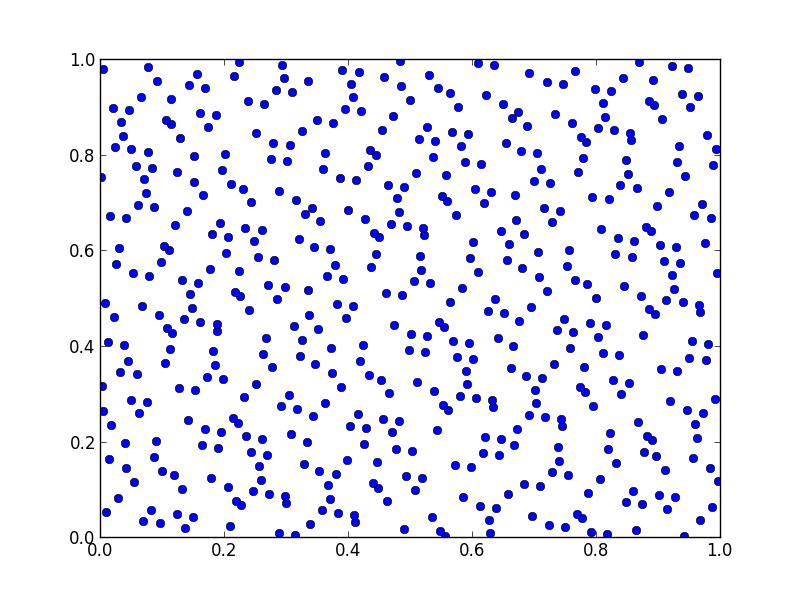
\includegraphics[width=0.6\linewidth]{../QuasiRandom1.png}
\captionof{figure}{Random numbers generated by the Halton algorithmus with numbers 3 and 5}
\end{center}

\begin{center}
\centering
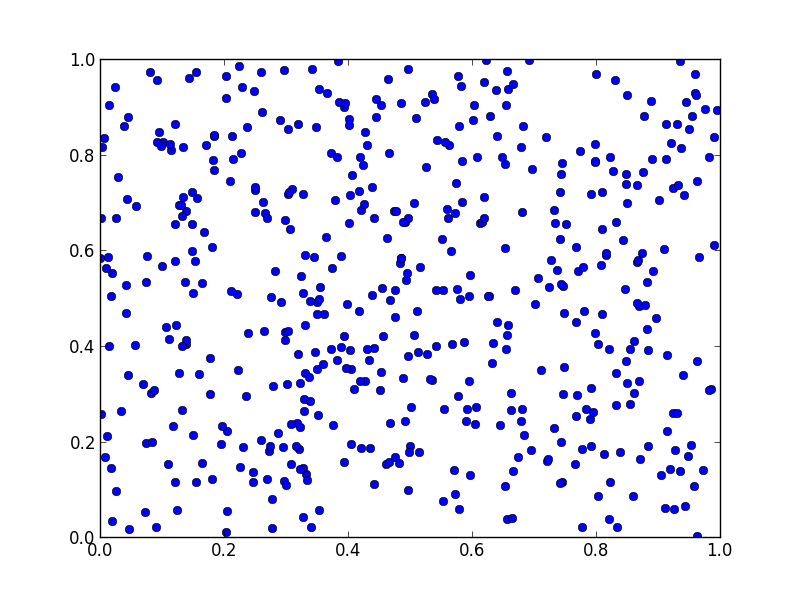
\includegraphics[width=0.6\linewidth]{../QuasiRandom2.png}
\captionof{figure}{Random numbers generated by the built-in random generator}
\end{center}

From the figures above we can see, that the quasi random numbers from the Halton algorithm have less clusters and seems to be more uniformly distributed.

\section*{Exercise 2}

The function \texttt{simulateRandomWalks} simulates 10000 random walks with 50 steps and prints the distribution of the total distance as well as the distance from the origin:

\lstinputlisting[language=Python]{../RandomWalk.py}

The plot of the distributions looks as follows:

\begin{center}
\centering
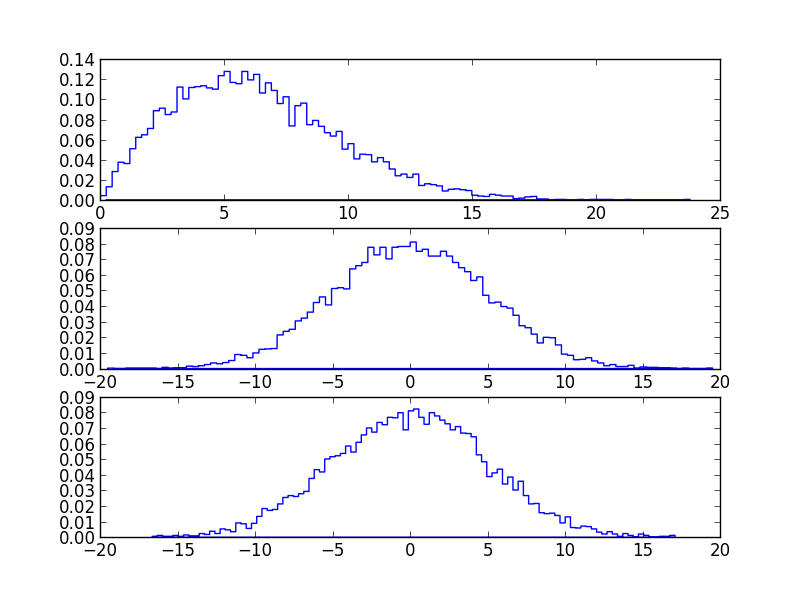
\includegraphics[width=0.6\linewidth]{../RandomWalk.png}
\captionof{figure}{Distribution of total distance (above) and distance from the origin.}
\end{center}

\section*{Exercise 3}

I use the fact that:

\begin{equation*}
\cos(x)=\frac{1}{2}(e^{ix}+e^{-ix})
\end{equation*}

With this, I can write:

\begin{eqnarray*}
\int\limits_{-\pi}^{\pi}\cos^{100}(x)dx&=&\int\limits_{-\pi}^{\pi}(\frac{1}{2}(e^{ix}+e^{-ix}))^{100}dx=\frac{1}{2^{100}}\sum\limits_{k=0}^{100}\binom{100}{k}\int\limits_{-\pi}^{\pi}e^{ikx}(-1)^{100-k}e^{-i(100-k)x}dx\\
&=&\frac{1}{2^{100}}\sum\limits_{k=0}^{100}\binom{100}{k}(-1)^{100-k}\int\limits_{-\pi}^{\pi}e^{ix(2k-100)}dx
\end{eqnarray*}

But if $k\neq 50$ we have $\int\limits_{-\pi}^{\pi}e^{ix(2k-100)}dx=0$ since we integrate just $N-2k$ times around the unit circle (in negative direction). Therefore:

\begin{eqnarray*}
\frac{1}{2^{100}}\sum\limits_{k=0}^{100}\binom{100}{k}(-1)^{100-k}\int\limits_{-\pi}^{\pi}e^{ix(2k-100)}dx&=&\frac{1}{2^{100}}\binom{100}{50}\int\limits_{-\pi}^{\pi}1dx\\
&=&\frac{1}{2^{100}}\binom{100}{50}2\pi
\end{eqnarray*}

Since we integrated over the domain $[-\pi,\pi]$, the average of $\cos^{100}(x)$ is just the integral divided by $2\pi$ which gives:

\begin{equation*}
\frac{\binom{100}{50}}{2^{100}}\approx 0.0796
\end{equation*}

\section*{Exercise 4}

The following script executes 100000 simulation where randomly $D$ or $M$ is reduced by 1 until either $D$ or $M$ is 0:

\lstinputlisting[language=Python]{../KSStatistics.py}

The output is a plot comparing the simulation with the Kolmogorov-Smirnov statistics:

\begin{center}
\centering
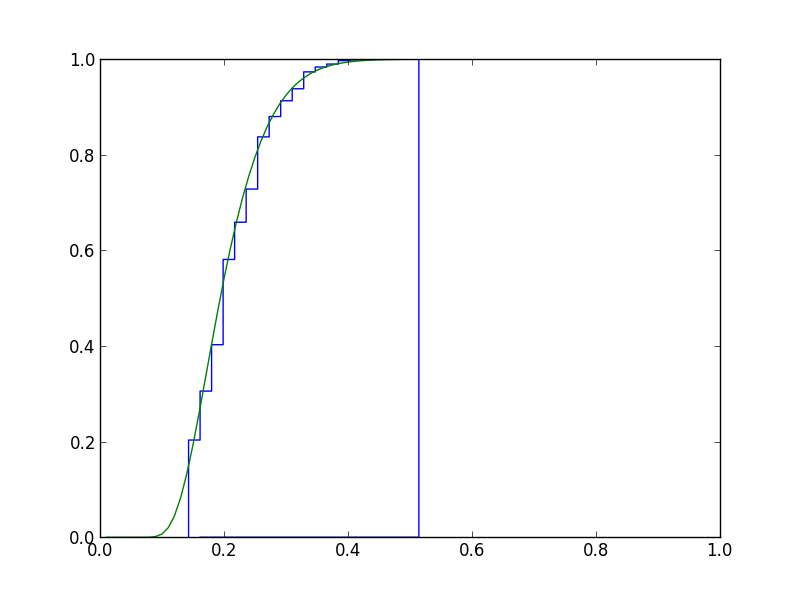
\includegraphics[width=0.6\linewidth]{../KSStatistics.png}
\captionof{figure}{The Kolmogorov-Smirnov statistics and an approximation by a simulation}
\end{center}

%% Bibliographie unter Verwendung von dinnat %%%%%%%%%%%%%%%%%%%%%%%%%%
%\setbibpreamble{Präambel}		% Text vor dem Verzeichnis
%\bibliographystyle{dinat}
%\bibliography{bibliographie}	% Sie benötigen einen *.bib-Datei

\end{document}
